% =====================================================================
% figures/operator-loop.tex
% Five-phase operator cycle T_0 -> T_1 -> T_2 -> T_3 -> T_4 with rho trace.
% Loaded by sections/03-phase-cycle.tex.
% =====================================================================
\begin{figure}[t]
\centering
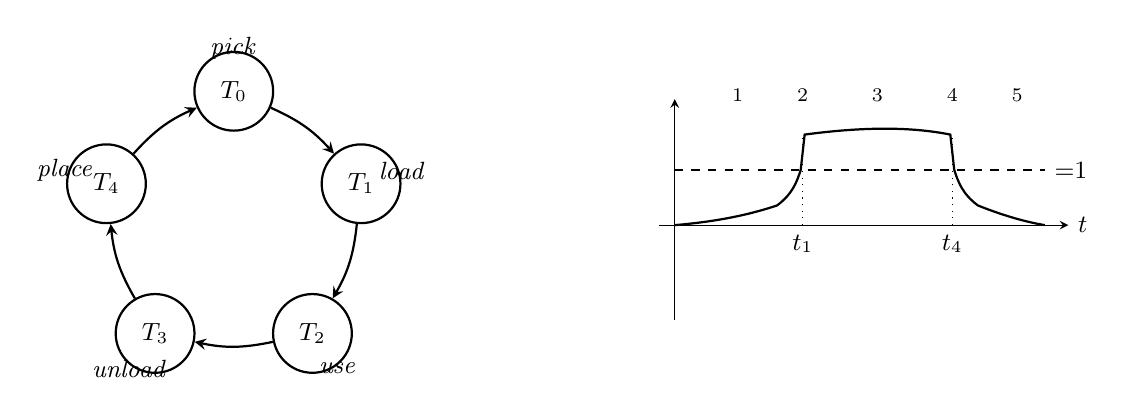
\begin{tikzpicture}[
    >=stealth,
    every node/.style={font=\small},
    op/.style={
      circle, draw, thick, minimum size=10mm, inner sep=1pt,
      fill=white
    },
    cycarrow/.style={->, thick}
  ]

  % --- Operator cycle (regular pentagon) ---
  \begin{scope}[shift={(-3.6,0)}]
    \def\R{1.7}
    \foreach \i/\name/\op in {
        0/pick/T_{0},
        1/load/T_{1},
        2/use/T_{2},
        3/unload/T_{3},
        4/place/T_{4}}
    {
      \pgfmathsetmacro{\ang}{90 - 72*\i}
      \node[op] (n\i) at (\ang:\R) {$\op$};
      \node at (\ang:\R+0.55) {\textit{\name}};
    }
    \draw[cycarrow] (n0) to[bend left=12] (n1);
    \draw[cycarrow] (n1) to[bend left=12] (n2);
    \draw[cycarrow] (n2) to[bend left=12] (n3);
    \draw[cycarrow] (n3) to[bend left=12] (n4);
    \draw[cycarrow] (n4) to[bend left=12] (n0);
  \end{scope}

  % --- rho trace (right inset) ---
  \begin{scope}[shift={(2.0,0)}]
    % axes
    \draw[->] (0,-1.2) -- (0,1.6) node[above] {$\rcontact$};
    \draw[->] (-0.2,0) -- (5.0,0) node[right] {$t$};

    % rho = 1 dashed line
    \draw[dashed] (0,0.7) -- (4.7,0.7) node[right] {$\rcontact{=}1$};

    % rho trace: low, jumps up at t1, plateau >1, drops at t4, low again
    \draw[thick]
      (0,0.0)
      .. controls (0.6,0.05) and (1.0,0.15) .. (1.3,0.25)
      .. controls (1.5,0.4) and (1.55,0.55) .. (1.6,0.7)
      -- (1.65,1.15)
      .. controls (2.4,1.25) and (3.0,1.25) .. (3.5,1.15)
      -- (3.55,0.7)
      .. controls (3.6,0.55) and (3.65,0.4) .. (3.85,0.25)
      .. controls (4.1,0.15) and (4.4,0.05) .. (4.7,0.0);

    % t1, t4 markers
    \draw[dotted] (1.625,0) -- (1.625,1.15);
    \draw[dotted] (3.525,0) -- (3.525,1.15);
    \node[below] at (1.625,0) {$t_{1}$};
    \node[below] at (3.525,0) {$t_{4}$};

    % phase labels along time axis
    \node[above, font=\scriptsize] at (0.8,1.45)  {1};
    \node[above, font=\scriptsize] at (1.625,1.45) {2};
    \node[above, font=\scriptsize] at (2.575,1.45) {3};
    \node[above, font=\scriptsize] at (3.525,1.45) {4};
    \node[above, font=\scriptsize] at (4.35,1.45) {5};
  \end{scope}

\end{tikzpicture}
\caption[Five-phase operator cycle with $\rcontact$ trace.]{
Left: directed cycle of the five phase operators
$\phaseop{0} \to \phaseop{1} \to \phaseop{2} \to \phaseop{3} \to
\phaseop{4} \to \phaseop{0}$, with each vertex labeled by its
phase name (\emph{pick}, \emph{load}, \emph{use}, \emph{unload},
\emph{place}). Right: schematic trace of the contact order
parameter $\rcontact$ along the cycle. The trajectory crosses
the level set $\rcontact = 1$ upward at the
contact-establishment time $t_{1}$ and downward at the release
time $t_{4}$, so that $\rcontact > 1$ on the open interior
$(t_{1}, t_{4})$ corresponding to phase 3 (use) and
$\rcontact < 1$ on the out-of-contact phases 1 (pick) and 5
(place). The diagram is structural: it depicts the combinatorial
type of every admissible pick--place trajectory, not a particular
realization.}
\label{fig:operator-loop}
\end{figure}
